Ahora que tenemos planificadas la gran mayoría de tareas principales y a más alto nivel, vamos a empezar con el desarrollo como tal de la aplicación. En esta sección presentaremos el logo de la app junto con el nombre y los diseños de las principales interfaces. 

\subsubsection{Logo de la aplicación y nombre}

Una de las primeras cosas en las que pensamos cuando escuchamos aplicación móvil es en el nombre y el logo de las grandes aplicaciones. En la época actual los logos tienen a ser minimalistas, simples y con colores pastel y suaves. Así mismo los nombres de las aplicaciones tienden a ser cortos, ya que los dispositivos móviles suelen tener un tamaño reducido y no se pueden meter frases largas. 

\subsubsection*{Logo}

Los dos diseños iniciales para el logo de la aplicación fueron los siguientes: 

\begin{multicols}{2}
    \begin{figure}[H]
        \centering
        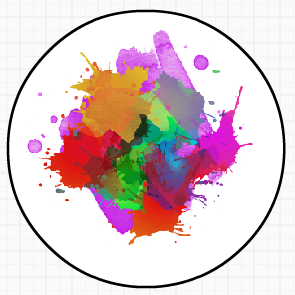
\includegraphics[scale=0.8]{imagenes/diseno/logo1.png}
        \caption{Diseño 1 del logo de la aplicación}
        \label{fig:logo1}
    \end{figure}
    
    \begin{figure}[H]
        \centering
        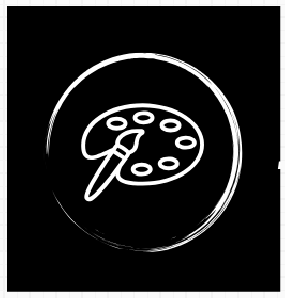
\includegraphics[scale=0.8]{imagenes/diseno/logo2.png}
        \caption{Diseño 1 del logo de la aplicación}
        \label{fig:logo2}
    \end{figure}
\end{multicols}

Pero después de una reunión con el cliente final, se llego a la conclusión de que el logo debería de ir mas por el estilo de la paleta:

\begin{figure}[H]
    \centering
    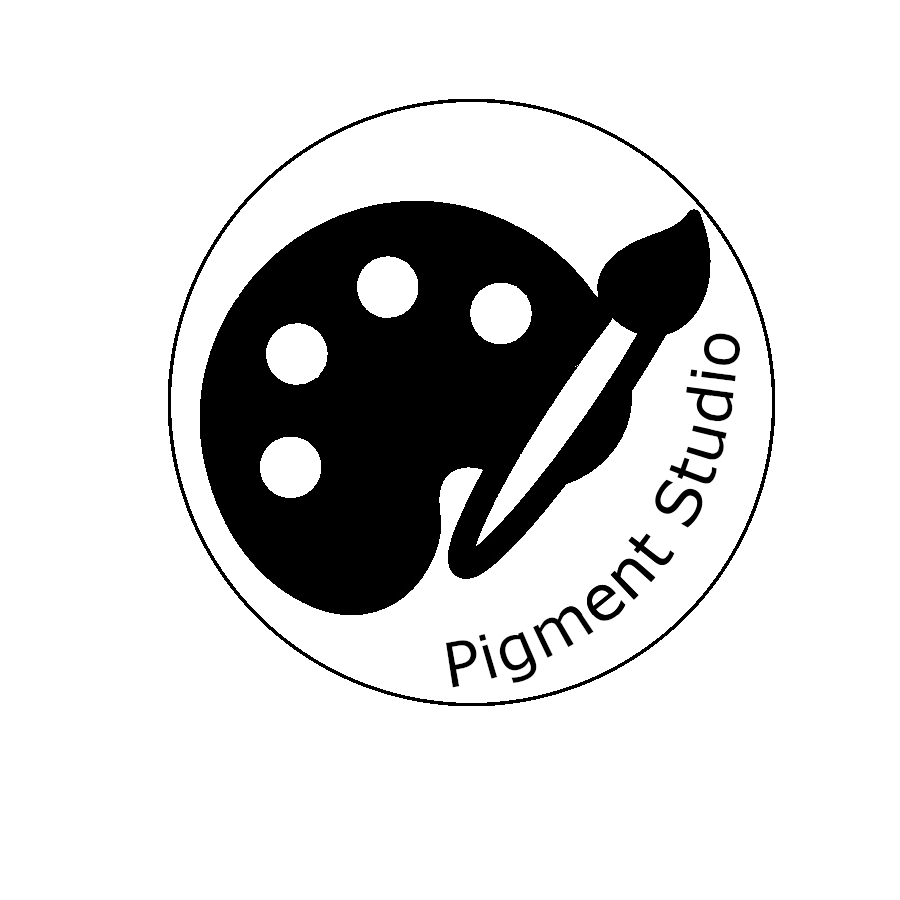
\includegraphics[scale=0.3]{imagenes/diseno/logo3.png}
    \caption{Diseño final del logo de la aplicación}
    \label{fig:logo3}
\end{figure}

\subsubsection*{Nombre}

En la sección anterior ya hemos dejado ver cual iba a ser el nombre de la aplicación. Una de las ideas iniciales era:
\begin{itemize}
    \item \textbf{PigemtsDB}: pero ni al cliente ni al tutor del TFG les convencía esta opción, ya que al contener la acortación DB, procedente de Data Base incluía unas connotaciones un poco más técnicas.
\end{itemize}

Al final se ha dejado como \textbf{Pigment Studio} ya que tiene un significado ligeramente más general y no restringe a ningún tipo de colectivos. 

Es un nombre corto y que haces una buena referencia a lo que el usuario se va a encontrar cuando abra la aplicaicón, que no es más que un estudio bastante avanzado y claro de los diferentes pigmentos que tenemos en el mundo. 

\subsubsection{Diseño de las primeras interfaces}

Una de las partes más críticas cuando estamos desarrollando aplicaciones que va a utilizar el usuario final es la interfaz que van a tener que usar. Va a ser una pantalla contra la que el usuario va a interactuar bastante a menudo, por lo tanto tiene que ser cómoda, clara y sencilla. Algunas de las normas que tienen que tener el diseño de interfaces para que el usuario tenga una buena experiencia (UX) las podemos encontrar en la siguiente lista \textcolor{red}{buscar en la bibliografía de IPC algo sobre el diseño de interfaces de usuario y citar un par de libros}: 
\begin{itemize}
   \item 
\end{itemize}